\documentclass[10pt]{article}
% Shared preamble for margin-stack prototypes.
% Mirrors the production geometry: 2.6cm-wide rungs, optional 0.3cm spine at
% x=2.85-3.15, \rmfamily labels (Palatino under the real build).
\usepackage{tikz}
\usetikzlibrary{positioning,calc,patterns,decorations.pathmorphing,decorations.pathreplacing}
\usepackage{xcolor}
\usepackage[paperwidth=20cm,paperheight=25cm,margin=8mm]{geometry}
\pagestyle{empty}

% Volume accents (from books/shared/tex/theme-colors-vol*.tex)
\definecolor{crimson}{HTML}{A51C30}      % vol1  Harvard Crimson
\definecolor{ethzblue}{HTML}{1F407A}     % vol2  ETH Zurich Blue
\definecolor{amethyst}{HTML}{581C87}     % vol3  Amethyst
\definecolor{emeraldpine}{HTML}{1A4D3E}  % vol4  Emerald Pine

% One rung. #1 y-bottom  #2 height  #3 label  #4 intensity 0-100  #5 accent
\newcommand{\protorung}[5]{%
  \ifnum#4=0
    \def\fillcol{black!5}\def\textcol{black!30}%
  \else
    \def\fillcol{#5!#4!white}%
    \ifnum#4>50 \def\textcol{white}\else \def\textcol{#5}\fi
  \fi
  \node[draw=white,line width=0.5pt,fill=\fillcol,minimum width=2.6cm,
        minimum height=#2 cm,anchor=south west,inner sep=0pt] (b) at (0,#1) {};
  \node[anchor=west,text=\textcol,font=\rmfamily\scriptsize\bfseries]
        at ($(b.west)+(0.12,0)$) {#3};
}

% Rung with a right-aligned secondary label (cadence, rate, count).
% #1 y  #2 h  #3 label  #4 right-label  #5 intensity  #6 accent
\newcommand{\protorungrt}[6]{%
  \ifnum#5=0
    \def\fillcol{black!5}\def\textcol{black!30}%
  \else
    \def\fillcol{#6!#5!white}%
    \ifnum#5>50 \def\textcol{white}\else \def\textcol{#6}\fi
  \fi
  \node[draw=white,line width=0.5pt,fill=\fillcol,minimum width=2.6cm,
        minimum height=#2 cm,anchor=south west,inner sep=0pt] (b) at (0,#1) {};
  \node[anchor=west,text=\textcol,font=\rmfamily\scriptsize\bfseries]
        at ($(b.west)+(0.12,0.09)$) {#3};
  \node[anchor=west,text=\textcol,font=\rmfamily\fontsize{4.6}{5}\selectfont,opacity=0.85]
        at ($(b.west)+(0.12,-0.12)$) {#4};
}

% Vertical cross-cutting spine at x=2.85..3.15 (vol1 data bar / vol3 trajectory).
% #1 y-bottom  #2 y-top  #3 word  #4 intensity  #5 accent
\newcommand{\protospine}[5]{%
  \fill[#5!#4!white,rounded corners=1.5pt] (2.85,#1) rectangle (3.15,#2);
  \pgfmathsetmacro{\midy}{(#1+#2)/2}
  \ifnum#4>50 \def\spinecol{white}\else \def\spinecol{#5}\fi
  \node[rotate=90,text=\spinecol,font=\rmfamily\fontsize{5}{6}\selectfont\bfseries]
        at (3.0,\midy) {#3};
}

% Caption under a prototype.
\newcommand{\protocap}[2]{%
  \begin{minipage}[t]{3.0cm}\raggedright
  \textbf{\footnotesize #1}\\[1pt]{\fontsize{6.5}{8}\selectfont #2}
  \end{minipage}}

% vol3-scale rung: 4.8pt label, matching tex/agent-stack-vol3.tex exactly.
\newcommand{\protorungsm}[5]{%
  \ifnum#4=0 \def\fillcol{black!5}\def\textcol{black!30}%
  \else \def\fillcol{#5!#4!white}%
    \ifnum#4>50 \def\textcol{white}\else \def\textcol{#5}\fi \fi
  \node[draw=white,line width=0.4pt,fill=\fillcol,minimum width=2.6cm,
        minimum height=#2 cm,anchor=south west,inner sep=0pt] (b) at (0,#1) {};
  \node[anchor=west,text=\textcol,font=\rmfamily\fontsize{4.8}{5.2}\selectfont\bfseries]
        at ($(b.west)+(0.12,0)$) {#3};
}
\newcommand{\protorungsmrt}[6]{%
  \ifnum#5=0 \def\fillcol{black!5}\def\textcol{black!30}%
  \else \def\fillcol{#6!#5!white}%
    \ifnum#5>50 \def\textcol{white}\else \def\textcol{#6}\fi \fi
  \node[draw=white,line width=0.4pt,fill=\fillcol,minimum width=2.6cm,
        minimum height=#2 cm,anchor=south west,inner sep=0pt] (b) at (0,#1) {};
  \node[anchor=west,text=\textcol,font=\rmfamily\fontsize{4.8}{5.2}\selectfont\bfseries]
        at ($(b.west)+(0.12,0.07)$) {#3};
  \node[anchor=west,text=\textcol,font=\rmfamily\fontsize{3.9}{4.4}\selectfont,opacity=0.85]
        at ($(b.west)+(0.12,-0.09)$) {#4};
}

\begin{document}
\noindent{\Large\bfseries Volume II margin stack --- current form and one addition}\\[2pt]
{\footnotesize A is what ships today (\texttt{\textbackslash mlfleetstackwithparts}, all 17 chapters):
eight rungs banded into four Part boxes. Shading is the \emph{compute infrastructure} chapter.
Note the stale comment in \texttt{.layout/tables/vol2/tables.tex} describes a different,
9-argument stack with a Data bar; that is not the macro the book calls.}\\[8mm]

\noindent
% ---------- A: current ----------
\begin{minipage}[t]{3.5cm}
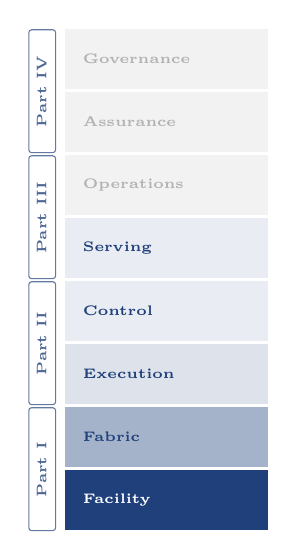
\begin{tikzpicture}
  \foreach \y/\n in {4.80/IV, 3.20/III, 1.60/II, 0.00/I} {
    \node[draw=ethzblue!70,line width=0.4pt,rounded corners=1pt,
          minimum width=0.34cm,minimum height=1.56cm,anchor=south west,inner sep=0pt]
          at (-0.45,\y) {};
    \node[rotate=90,text=ethzblue,opacity=0.8,
          font=\rmfamily\fontsize{4.6}{5}\selectfont\bfseries] at (-0.28,\y+0.78) {Part~\n};
  }
  \protorungsm{5.60}{0.78}{Governance}{0}{ethzblue}
  \protorungsm{4.80}{0.78}{Assurance}{0}{ethzblue}
  \protorungsm{4.00}{0.78}{Operations}{0}{ethzblue}
  \protorungsm{3.20}{0.78}{Serving}{10}{ethzblue}
  \protorungsm{2.40}{0.78}{Control}{10}{ethzblue}
  \protorungsm{1.60}{0.78}{Execution}{15}{ethzblue}
  \protorungsm{0.80}{0.78}{Fabric}{40}{ethzblue}
  \protorungsm{0.00}{0.78}{Facility}{100}{ethzblue}
\end{tikzpicture}\\[3mm]
\protocap{A. Current (ships today)}{Eight rungs, four Part boxes. The banding is already the device image~4 uses; vol2 got there first.}
\end{minipage}\hfill
% ---------- B: + data bar ----------
\begin{minipage}[t]{3.9cm}
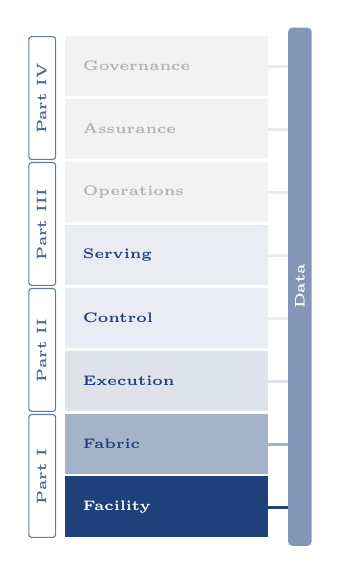
\begin{tikzpicture}
  \foreach \y/\n in {4.80/IV, 3.20/III, 1.60/II, 0.00/I} {
    \node[draw=ethzblue!70,line width=0.4pt,rounded corners=1pt,
          minimum width=0.34cm,minimum height=1.56cm,anchor=south west,inner sep=0pt]
          at (-0.45,\y) {};
    \node[rotate=90,text=ethzblue,opacity=0.8,
          font=\rmfamily\fontsize{4.6}{5}\selectfont\bfseries] at (-0.28,\y+0.78) {Part~\n};
  }
  \protorungsm{5.60}{0.78}{Governance}{0}{ethzblue}
  \protorungsm{4.80}{0.78}{Assurance}{0}{ethzblue}
  \protorungsm{4.00}{0.78}{Operations}{0}{ethzblue}
  \protorungsm{3.20}{0.78}{Serving}{10}{ethzblue}
  \protorungsm{2.40}{0.78}{Control}{10}{ethzblue}
  \protorungsm{1.60}{0.78}{Execution}{15}{ethzblue}
  \protorungsm{0.80}{0.78}{Fabric}{40}{ethzblue}
  \protorungsm{0.00}{0.78}{Facility}{100}{ethzblue}
  \foreach \lint/\ypos in {100/0.39, 40/1.19, 15/1.99, 10/2.79, 10/3.59, 0/4.39, 0/5.19, 0/5.99} {
    \ifnum\lint=0 \def\wirecol{black!8}\else \edef\wirecol{ethzblue!\lint}\fi
    \draw[\wirecol,line width=1.0pt] (2.6,\ypos) -- (2.85,\ypos);
  }
  \protospine{-0.10}{6.48}{Data}{55}{ethzblue}
\end{tikzpicture}\\[3mm]
\protocap{B. + Data bar}{vol1's device, restored. Data is cross-cutting at fleet scale too, and the wires show which layers touch it.}
\end{minipage}\hfill
\begin{minipage}[t]{5.2cm}\raggedright
\textbf{\footnotesize Correction to my earlier read}\\[2pt]
{\fontsize{7}{9}\selectfont
I said vol2's Security and Governance were flattened into the ladder as pseudo-strata.
That was drawn from the stale doc comment. The macro the chapters actually call already
bands Assurance and Governance together as Part~IV, which is the right treatment. vol2's
stack does not have the defect I described.\\[4pt]
The one real gap is the Data bar: vol1 carries it, vol2 dropped it when the 9-argument
form was replaced by the 8-argument part-banded form. Whether data still deserves a
cross-cutting bar at fleet scale is your call, not a defect.}
\end{minipage}
\end{document}
